
\section{Light Curtain only Experiments}

Can we estimate depth using just the Light Curtain? In this initial baseline, we attempt to track the Uncertainty Field (UF) depth error by computing the RMSE error metric $\sqrt{\stackrel[i=1]{n}{\sum}\frac{\left(\mathbb{E}\left(UF\left(u,q\right)\right)-\mathbf{d_{gt}}(u)_{i}\right)^{2}}{n}}$ against the ground truth. We use 3 scenarios: One in a KITTI driving scene using the LC simulator (a), one indoors in the basement using the both a simulated and real Light Curtain (b), and lastly in various outdoor driving scenes with the real device (c0/c1/c2). 

\begin{figure}[h]
   \centering
   \begin{minipage}{0.5\textwidth}
       \centering
       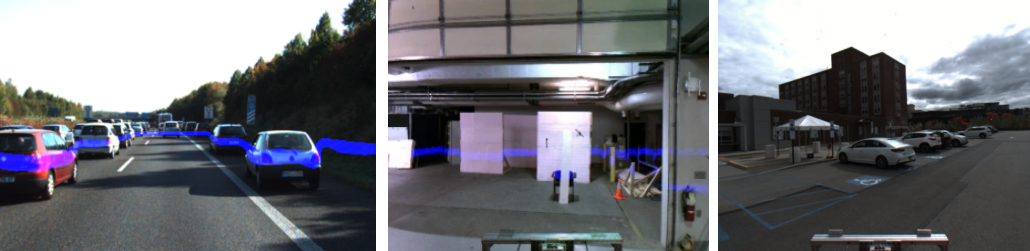
\includegraphics[width=1.0\textwidth]{figures/exp.png}
   \end{minipage}\hfill
   \centering
   \caption{Scenarios (a), (b), (c) from left to right}
   \label{fig:exp}
\end{figure}

\textbf{Planar Sweep:} A simple sanity check between simulation and the real sensor involves involves performing a uniform sweep across the scene in (b). As seen in Fig.~\ref{fig:planarsweep}, our simulated Light Curtain (LC) is able to reasonably match the real device. We also demonstrate how decreasing the steps the curtain takes reduces runtime but increases RMSE. Results seen in Tab.~\ref{table:t1}
 
\begin{figure}
   \centering
   \begin{minipage}{0.4\textwidth}
       \centering
       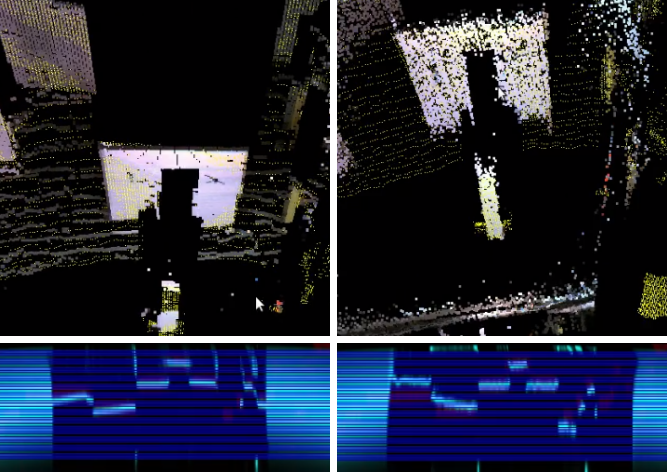
\includegraphics[width=1.0\textwidth]{figures/sweep.png}
   \end{minipage}\hfill
   \centering
   \caption{Doing a simple planar sweep of the Light Curtain (LC) across a scene. Colored pointcloud is the estimated depth, and Lidar ground truth in yellow. \textbf{Left:} LC simulated from the Lidar Depth. \textbf{Right:} Using the real LC}
   \label{fig:planarsweep}
\end{figure}

%\vspace{-.1in}
\begin{table}[h]
   \centering
   \resizebox{0.7\linewidth}{!}{
   \begin{tabular}{|l|l|l|}
   \hline
    Policy&  Runtime/s&  RMSE/m\\ \hline
    Sweep 50 $\mathbf{C}$ Step 0.25m (Sim) &-  &1.156  \\ \hline
    Sweep 25 $\mathbf{C}$ Step 0.5m  (Sim) &-  &1.374  \\ \hline
    Sweep 50 $\mathbf{C}$ Step 0.25m (Real) &2  &1.284  \\ \hline
    Sweep 25 $\mathbf{C}$ Step 0.5m  (Real) &1  &1.574  \\ \hline
    Sweep 12 $\mathbf{C}$ Step 1.0m (Real) &0.5  &1.927  \\ \hline
   \end{tabular}}

   \caption{We demonstrate corroboration between simulated and real Light Curtain, and we show that sampling the scene further by placing more curtains results in better depth}
   \label{table:t1}
   %\vspace{.1in}
   
%    \resizebox{0.7\linewidth}{!}{
%     \begin{tabular}{|l|l|l|}
%     \hline
%      Policy&  Runtime/s&  RMSE/m\\ \hline
%      Sweep $\mathbf{C}$ Step 0.25m (Dyn) &2  &1.276  \\ \hline
%      Sweep $\mathbf{C}$ Step 0.5m  (Dyn) &1  &1.532  \\ \hline
%      Sweep $\mathbf{C}$ Step 1.0m (Dyn) &0.5  &2.013  \\ \hline
%      Sweep $\mathbf{C}$ Step 0.25m (Fixed) &2  &1.218  \\ \hline
%      Sweep $\mathbf{C}$ Step 0.5m  (Fixed) &1  &1.658  \\ \hline
%      Sweep $\mathbf{C}$ Step 1.0m (Fixed) &0.5  &2.290  \\ \hline
%     \end{tabular}} 
   
%    \caption{$\sigma_{c}$ in our model $P\left(\mathbf{d}_{u,v}^{c_{k}}\right)$ being dynamic as a function of curtain thickness as opposed to being fixed, results in better depth estimates}
%    \label{table:t2}
\end{table}

% \textbf{Effect of Dynamic Sigma:} Earlier, we had noted how $\sigma(u,v,d_{u,v}^{c})$ defined for each $c_{k}$ measurement in $P\left(\mathbf{d}_{u,v}^{c_{k}}\right)$ is a function of the thickness of the curtain. We also experiment by making $\sigma(u,v,d_{u,v}^{c})$ fixed. We observe that it being a function of the curtain thickness is critical to better performance over larger steps/placements. Results in Tab.~\ref{table:t2}

% %\vspace{-.1in}
% \noindent
% \begin{table}[h]
%    \centering
%    \resizebox{0.7\linewidth}{!}{
%    \begin{tabular}{|l|l|l|}
%    \hline
%     Policy&  Runtime/s&  RMSE/m\\ \hline
%     Sweep $\mathbf{C}$ Step 0.25m (Dyn) &2  &1.276  \\ \hline
%     Sweep $\mathbf{C}$ Step 0.5m  (Dyn) &1  &1.532  \\ \hline
%     Sweep $\mathbf{C}$ Step 1.0m (Dyn) &0.5  &2.013  \\ \hline
%     Sweep $\mathbf{C}$ Step 0.25m (Fixed) &2  &1.218  \\ \hline
%     Sweep $\mathbf{C}$ Step 0.5m  (Fixed) &1  &1.658  \\ \hline
%     Sweep $\mathbf{C}$ Step 1.0m (Fixed) &0.5  &2.290  \\ \hline
%    \end{tabular}}
%    \caption{$\sigma_{c}$ in our model $P\left(\mathbf{d}_{u,v}^{c_{k}}\right)$ being dynamic as a function of curtain thickness as opposed to being fixed, results in better depth estimates}
%    \label{table:t2}
% \end{table}

\textbf{Effect of Inverting Gaussian Model:} Our Observation Model ensures that the sensor distribution tends to an Inverted Gaussian when intensities are low, instead of a Uniform distribution. We see significantly improved performance when low intensities tend to an Inverted Gaussian instead. Results seen in Fig.~\ref{fig:figure01} ~\ref{fig:invgau}

\begin{figure}[h]
    \centering
    \begin{minipage}{0.5\textwidth}
        \centering
        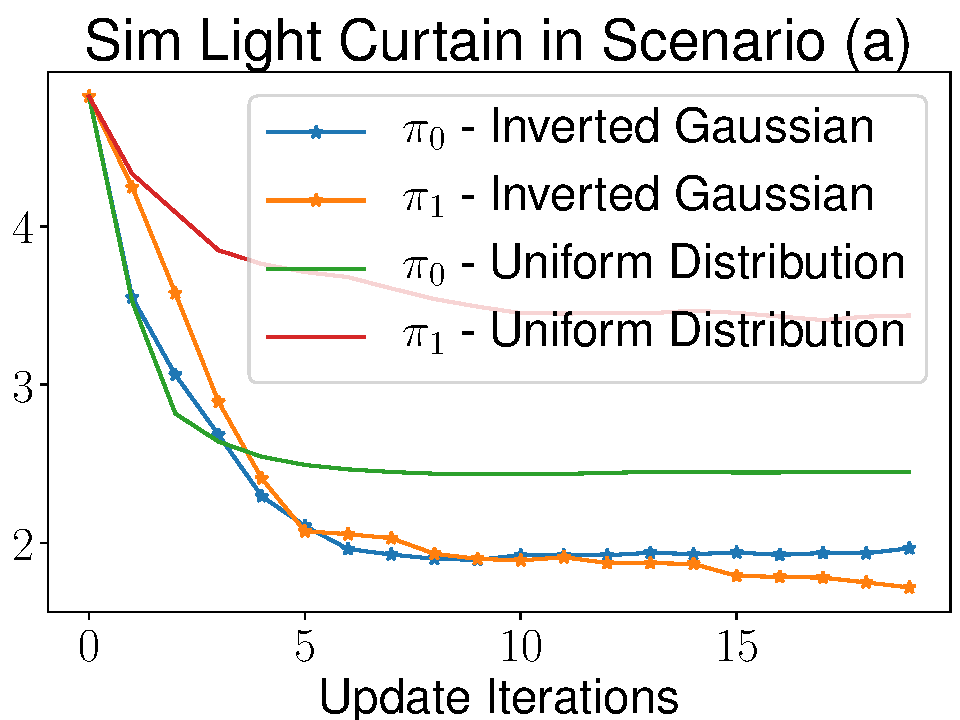
\includegraphics[width=0.49\textwidth]{figures/Figure_1.pdf}
        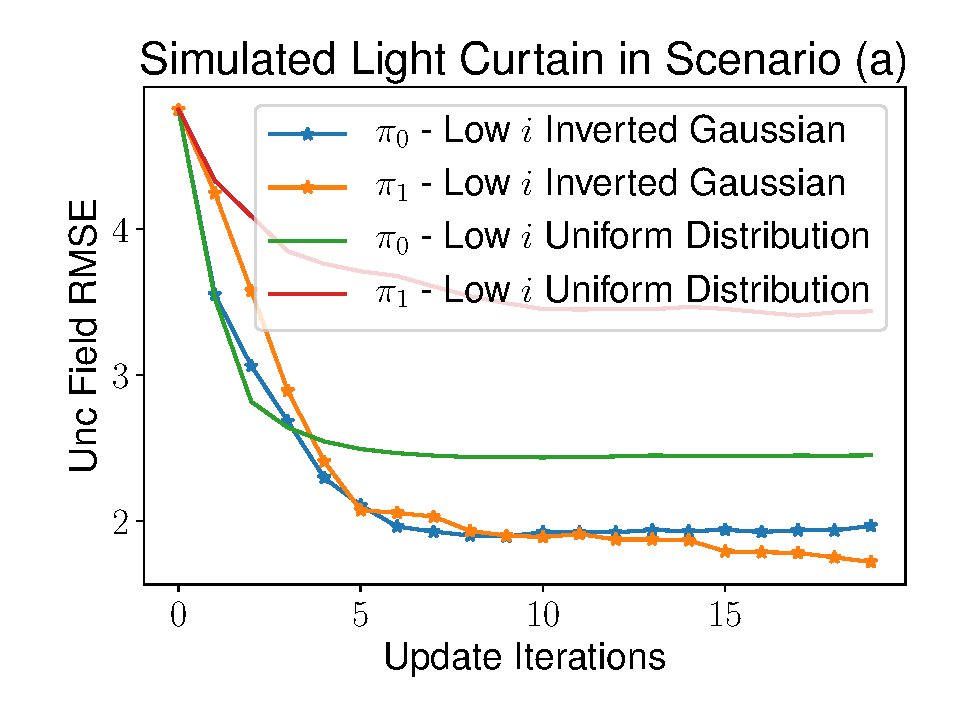
\includegraphics[width=0.49\textwidth]{figures/Figure_0.pdf}
    \end{minipage}\hfill
    \centering
    \caption{We get better depth estimate over increased sampling iterations, when low intensity values sampled by the light curtain generate an Inverted Gaussian Depth Distribution, as opposed to a uniform one in both simulation and real world experiments}
    \label{fig:figure01}
\end{figure}

 \begin{figure}[h]
    \centering
    \begin{minipage}{0.5\textwidth}
        \centering
        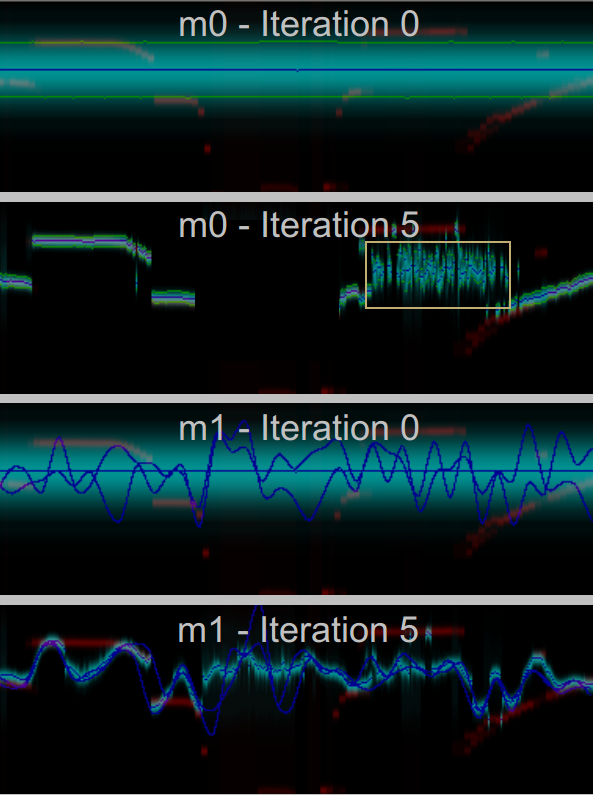
\includegraphics[width=0.49\textwidth]{figures/InvGau.png}
        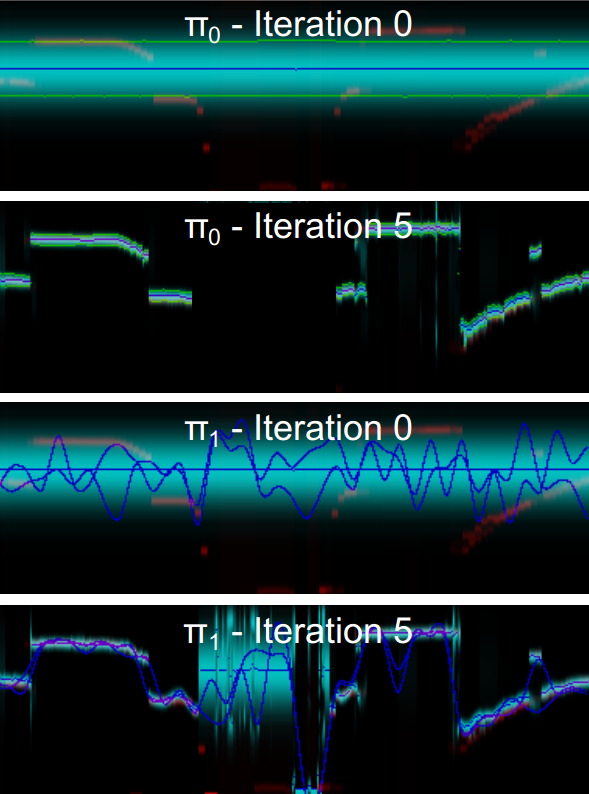
\includegraphics[width=0.49\textwidth]{figures/Uniform.png}
    \end{minipage}\hfill
    \centering
    \caption{Looking at the top-down Uncertainty Field (UF), we see per pixel distributions in Blue and the GT in Red. We start with a gaussian prior with a large $\sigma$, take measurements and apply the bayesian update. \textbf{Left:} Policies $\pi_{0}$ and $\pi_{1}$ where low intensities result in no information (Uniform Distribution). \textbf{Right:} Where low intensities result in an Inverted Gaussian based on our Sensor Model}
    \label{fig:invgau} 
\end{figure}

 \textbf{Effect of Placing more Curtains:} In both policies, placing more light curtains results in much faster convergence, at the cost of increased runtime. Results seen in Fig.~\ref{fig:figure34}

\begin{figure}[h]
    \centering
    \begin{minipage}{0.5\textwidth}
        \centering
        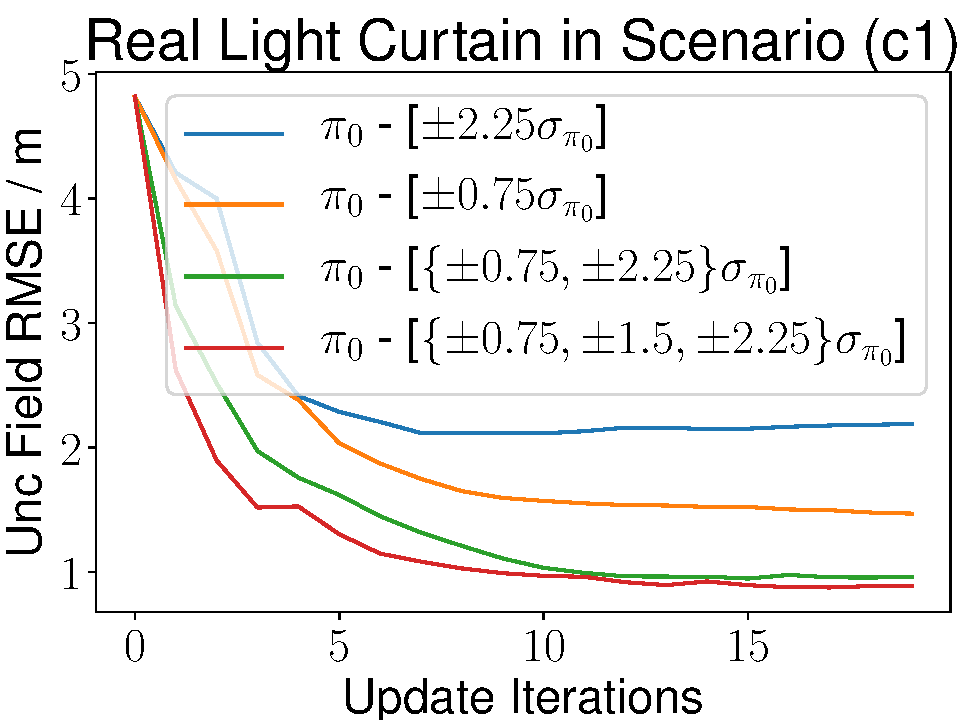
\includegraphics[width=0.49\textwidth]{figures/Figure_3.pdf}
        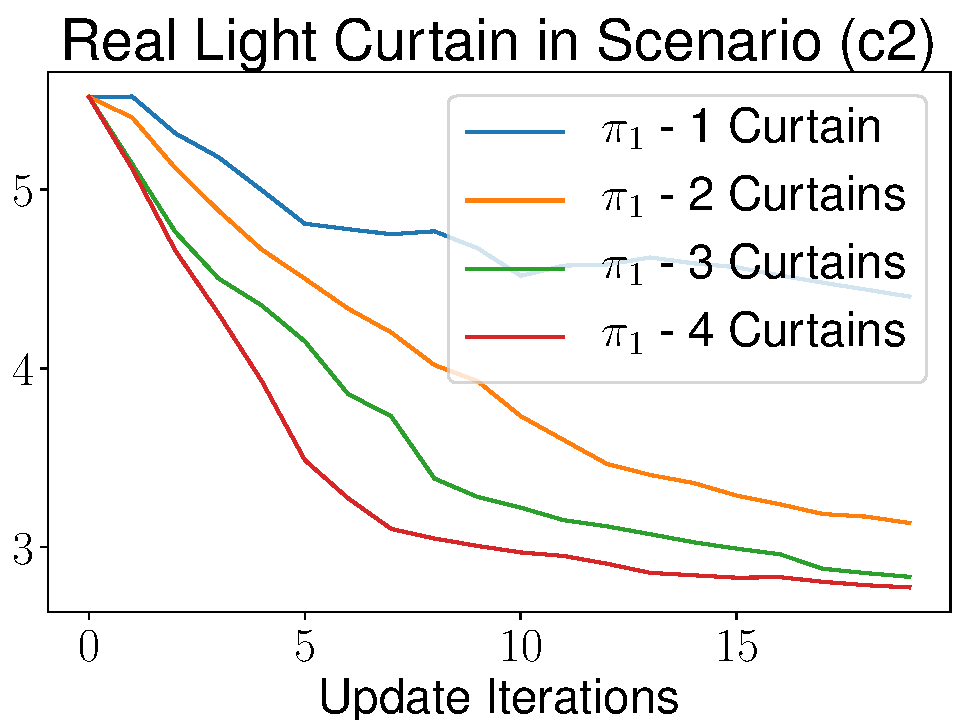
\includegraphics[width=0.49\textwidth]{figures/Figure_4.pdf}
    \end{minipage}\hfill
    \centering
    \caption{Placing more curtains results in faster convergence to the ground truth at the cost of runtime per iteration}
    \label{fig:figure34}
\end{figure}

% While this is a reasonable approach to estimating depth, it is also slow, as it requires placing many curtains. 

